% 第三章正文主版本；历史Markdown不再同步。
\chapter[任务相关响应下的CPU--NPU热约束调度建模与求解]{任务相关响应下的CPU--NPU\\热约束调度建模与求解}
\label{chap:model}

\section{本章引言}

面向xxx，针对xxx的问题，提出了一种xxx的算法。

本章结构如下：第3.2节建立系统模型，包括任务模型、处理器模型和执行模式；第3.3节建立功耗与温度模型，包括执行状态和功率模型、系统能耗模型以及瞬态温度模型；第3.4节给出问题定义；第3.5节对xxx问题进行分析并给出形式化表达；第3.6节介绍基于xxx的混合整数线性规划方法xxx-MILP求解流程；第3.7节给出仿真结果与分析；第3.8节总结本章工作。

\begin{table}[!htbp]
\centering\small
\caption{四Stage划分与条件性设备支持}\label{tab:stage-support}
\begin{tabular}{@{}p{2.0cm}p{2.8cm}p{4.0cm}p{4.5cm}@{}}
\toprule
Stage & 算子范围，含端点 & 作者报告的CPU--NPU支持子集 & 在本章实例中的作用 \\
\midrule
S0 & 0 & CPU & 请求首阶段，完整保留 \\
S1 & 1--65 & CPU、所报告后端条件下的NPU & 可替代设备映射阶段 \\
S2 & 66--265 & CPU & 依赖S1输出的CPU阶段 \\
S3 & 266 & CPU & 产生最终输出，决定请求完成 \\
\bottomrule
\end{tabular}
\end{table}

\begin{figure}[htbp]
\centering
\begin{tikzpicture}[node distance=5mm,box/.style={draw,rounded corners,align=center,text width=8cm,minimum height=8mm,font=\small},>=Latex]
\node[box] (i) {模型输入：$1\times320\times320\times3$，UINT8};
\node[box,below=of i] (s0) {S0：CPU，算子0};
\node[box,below=of s0] (s1) {S1：CPU或指定NPU，算子1--65};
\node[box,below=of s1] (s2) {S2：CPU，算子66--265};
\node[box,below=of s2] (s3) {S3：CPU，算子266};
\node[box,below=of s3] (o) {模型输出};
\foreach \a/\b in {i/s0,s0/s1,s1/s2,s2/s3,s3/o} \draw[->] (\a)--(\b);
\end{tikzpicture}
\caption{四Stage结构及条件性设备支持。各Stage覆盖全部267个算子且不重复；箭头为静态数据依赖。多个请求复制同一任务图并共享资源。}
\label{fig:stage-structure}
\end{figure}


上述材料锚定的是任务结构和作者报告的设备支持能力，而不是本章的性能测量。它来自作者后续分区工件，不等同于Band论文图6的实验流程。本文保留四个Stage及其依赖，用两个同模型请求说明跨请求资源竞争；相同Stage在两个请求中使用相同响应参数，不通过请求编号人为制造性能差异。

\subsection{固定执行单元与频率控制}

平台包含多个CPU执行单元和一个NPU。CPU单元集合记为\(\mathcal U_C\)，NPU记为\(u_N\)，全部执行单元组成\(\mathcal U=\mathcal U_C\cup\{u_N\}\)。一个CPU单元可以表示一个核，也可以表示占用预先固定核集合的工作线程组；各CPU单元的占核集合不重叠。每个单元同一时刻只能执行一个Stage，Stage执行期间不抢占、不迁移。单元内部使用多少线程已经固定，不属于本文的优化变量。NPU采用固定服务模式，同一时刻执行一个Stage，但允许与CPU并发。

CPU频率由频率域控制。频率域是共享同一频率设置的一组CPU单元，记域集合为\(\mathcal D\)，映射\(h:\mathcal U_C\to\mathcal D\)给出各单元所属域，\(F_\delta\)给出域\(\delta\)的合法频点。当同域的不同单元同时运行时，其频率必须一致；只有该域的Stage全部完成后，才能切换到另一频率。因而，使用不同CPU单元并不必然意味着可以独立调频。不同域的频率则可分别选择，域结构作为平台输入给定。

贯穿实例采用两个对称CPU单元和一个共享频率域。假设两个请求的S2采用高频，而S3适合低频，则先完成S2的请求可能仍需等待另一请求的S2结束，随后才能执行低频S3。这种等待并非数据依赖直接要求，而是共享频率控制产生的合法性要求。另一方面，两个采用相同频率的S2可以在不同单元上错开重叠，不应被误写成整个CPU只能串行执行。

对称单元与实际硬件需要区分。作者测试中的CPU worker采用3线程BIG和4线程LITTLE配置\cite{source5}；本文将CPU支持类别展开为两个对称固定单元，是用于机制分析的研究假设，不复现这两个worker的性能。一般模型保留合法单元及频率域作为输入，本章实例不额外引入异构CPU或可变核组。

\subsection{任务相关执行模式}

一个执行模式同时回答“在哪里执行”和“以何种频率执行”。Stage \(i\)的有限合法模式集合记为\(M_i\)。模式\(m\in M_i\)包含执行单元\(u(m)\)、CPU频率\(\nu(m)\)、执行时长\(d_i(m)>0\)以及活动增量功率\(Q_i(m)\ge0\)。CPU模式的频率属于\(F_{h(u(m))}\)；NPU模式使用固定服务标记，不引入NPU调频决策。不支持的设备组合不进入\(M_i\)，必需Stage若没有合法模式，则该请求不可执行。

模式表既可以来自匹配测量，也可以由显式响应函数生成。为解释频率响应的差异，令\(x=f/F_{\rm ref}\)为相对于参考频率\(F_{\rm ref}\)的无量纲频率，\(\bar d_i\)为参考时长，可比较反比模型I与任务相关模型R：
\begin{equation}
\widehat d_i^I(x)=\frac{\bar d_i}{x},\qquad
\widehat d_i^R(x)=\bar d_i\left[(1-\alpha_i)+\frac{\alpha_i}{x}\right].
\label{eq:ch3-1}
\end{equation}
式中，\(\alpha_i\in[0,1]\)表示该说明性模型中随频率缩放的时间比例。\(\alpha_i=1\)时两种刻画相同；\(\alpha_i\)较小时，降低频率导致的时间增长较小。对\(0<x\le1\)，两者之差为\(\bar d_i(1-\alpha_i)(1/x-1)\ge0\)。因此，在活动功率相同的条件下，两者对低频模式的能量估计也可能不同。是否进一步改变系统选择，还取决于模式能否满足后继和期限要求。

本章采用Stage相关模式表，使执行时长同时进入能耗、资源占用、依赖和温度评价。只修改能量而保留原占用时间，会使同一模式在不同约束中具有矛盾含义。式\eqref{eq:ch3-1}仅用于解释和构造后续条件性对照；一般模型不要求所有Stage遵循该函数，也不从算子数量或单个时延点推断\(\alpha_i\)。服务器应用的响应研究\cite{source2}提供了区分响应的依据，其参数不直接作为端侧Stage参数。

这里对Zhou模型的调整限定于执行时间假设。原研究还包含任务活动差异和温度相关泄漏\cite{source1}；本章在采用任务相关时长的同时，使用模式内恒定活动功率，不保留温度相关泄漏。因此本文不是对原完整模型逐项精细化，而是在共同功率边界下隔离时长刻画的决策影响。

三个层次的映射含义也需分清。交换两个对称CPU的全部编号只是标签替换；将两个Stage分配到同一或不同CPU单元，会改变串行与并发机会；将S1从CPU转移到NPU，则同时改变执行设备、响应和注热位置。本文研究后两类选择，不把对称编号变化当作异构映射或热点迁移收益。

\section{功耗与温度模型}

执行模式给出了阶段时长和活动功率，但系统能耗还包含任务未运行时持续存在的公共部分；温度则取决于功率随时间的分布。本节先建立统一的功率计量，再描述功率轨迹如何产生温度，为后续约束提供共同评价口径。

\subsection{运行状态与系统能耗}

设Stage \(i\)选用模式\(m_i\)，启动时刻为\(s_i\)。其结束时刻、半开执行区间和运行指示分别为
\begin{equation}
b_i=s_i+d_i(m_i),\qquad I_i=[s_i,b_i),\qquad z_i(t)=\mathbf1_{I_i}(t).
\label{eq:ch3-2}
\end{equation}
半开区间表示Stage在结束时刻已经释放资源，后继可在该时刻开始。记完整模式配置为\(m=(m_i)_{i\in V}\)，启动向量为\(s=(s_i)_{i\in V}\)。给定二者，全部运行状态和功率事件即可确定。



设\(p_C^0\)为全部CPU单元的聚合空闲功率，\(p_N^0\)为NPU空闲功率，\(P_{\rm ext}\)为热边界外恒定公共功率，三者均非负。节点注热和系统功率定义为

\begin{equation}
\begin{aligned}
p_C(t)&=p_C^0+\sum_{i:u(m_i)\in\mathcal U_C}Q_i(m_i)z_i(t),\\
p_N(t)&=p_N^0+\sum_{i:u(m_i)=u_N}Q_i(m_i)z_i(t),\\
P_{\rm base}&=p_C^0+p_N^0+P_{\rm ext},\qquad
P_{\rm sys}(t)=p_C(t)+p_N(t)+P_{\rm ext}.
\end{aligned}
\label{eq:ch3-9}
\end{equation}

CPU活动增量按所有运行Stage求和，聚合空闲项只计一次。即使某方案不使用NPU，其空闲功率仍计入窗口。\(Q_i\)是相对于共同基准的活动增量，不能直接用未扣除公共部分的整机功率代替；只在任务活动期间出现的固定开销属于\(Q_i\)，不属于全窗口基准。

每个Stage在窗口内执行一次，故积分得到

\begin{equation}
E(m,s)=\int_0^W P_{\rm sys}(t)\,\mathrm dt
=P_{\rm base}W+\sum_{i\in V}Q_i(m_i)d_i(m_i)
\equiv E(m).
\label{eq:ch3-10}
\end{equation}

固定配置下，各Stage活动能量和窗口基准能量均固定。等待与重排改变功率出现的时刻，但不改变其积分。这一性质同时依赖固定窗口、恒定基准、固定模式响应和零额外开销，不意味着等待一定可行或一定降温。


例如，两个CPU单元分别执行请求A与B的Stage时，CPU节点功率等于一次聚合空闲功率加两个活动增量。如果B转而使用NPU，则其增量计入NPU节点；CPU的公共空闲项不会因此重复增加，NPU未被选用时的空闲项也不会自动消失。这种统一计量使串行、并发和不同设备映射可以在相同窗口内比较。

\subsection{瞬态温度与连续安全约束}

热阻热容（Resistance--Capacitance，RC）网络用热容表示储热能力，用导热系数表示热量流向环境或其他节点的能力。因而温度不会在功率改变时瞬间跳变，而会受此前热状态影响。本文将CPU和NPU分别视为聚合热节点。设环境温度\(T_a\)恒定，温升向量\(\theta(t)=[T_C(t)-T_a,T_N(t)-T_a]^{\mathsf T}\)，注热向量\(p(t)=[p_C(t),p_N(t)]^{\mathsf T}\)。热容与导热矩阵为

\begin{equation}
C_{\rm th}=\operatorname{diag}(C_C,C_N),\qquad
G=\begin{bmatrix}g_C+g&-g\\-g&g_N+g\end{bmatrix},
\quad C_C,C_N>0,\quad g_C,g_N>0,\quad g\ge0.
\label{eq:ch3-11}
\end{equation}

\(g_C,g_N\)表示节点对环境导热，\(g\)表示节点间耦合导热，单位为W/K。对非零向量\(v\)，有\(v^{\mathsf T}Gv=g_Cv_C^2+g_Nv_N^2+g(v_C-v_N)^2>0\)。因此\(G\)正定，\(-C_{\rm th}^{-1}G\)与负定对称矩阵相似，系统渐近稳定。\(g=0\)是合法无耦合特例，而非另一个热模型。

温度由确定的动力学和入口状态生成：

\begin{equation}
C_{\rm th}\dot\theta(t)=-G\theta(t)+p(t),\qquad
\theta(0)=[T_C^0-T_a,T_N^0-T_a]^{\mathsf T}.
\label{eq:ch3-12}
\end{equation}

\begin{equation}
T_a+\theta_n(t)\le T_n^{\max},\qquad n\in\{C,N\},\quad \forall t\in[0,W].
\label{eq:ch3-13}
\end{equation}

式\eqref{eq:ch3-9}中的边界内电功率作为对应节点注热，是本章明确采用的热边界假设。\(P_{\rm ext}\)只计系统能量，不任意注入CPU；若实际外部热源显著影响这两个节点，就需要扩展边界。CPU聚合节点无法区分按核热点，因此改变对称CPU标签不能被解释为热点迁移收益。

设\(A_T=-C_{\rm th}^{-1}G\)。在长度为\(\tau\)的恒功率段内，入口状态\(\theta(t_0)\)精确传播为

\begin{equation}
\theta(t_0+\tau)=e^{A_T\tau}\theta(t_0)
+\int_0^\tau e^{A_T(\tau-\xi)}C_{\rm th}^{-1}p\,\mathrm d\xi.
\label{eq:ch3-14}
\end{equation}

全部启动和结束事件划分恒功率段。连续温度评价需检查段端点以及内部驻点；只在启动网格或Stage结束处取样不足以保证式\eqref{eq:ch3-13}。初温只在窗口入口给定，等待时温度继续传播，不能在每次派发时重置。最后一个任务完成后的空闲尾段仍计入评价，耦合可能使某节点在自身停止活动后继续升温。

数学约束与计算判定需要分开：模型要求全过程不超过上限；数值评价应报告运算误差和边界未分辨状态。采样或ODE交叉核对能够检查实现，却不能自动替代全段峰值保证。本章安全结论限定在\([0,W]\)，不保证窗口之后或重复连续运行安全。


这一模型解释了能量相同的安排为何可能具有不同温度。并发会使若干活动增量在同一时段叠加；错开执行则改变散热与后续注热的先后关系。由于两个节点还会交换热量，不能只比较阶段总能量或CPU自身功率判断峰温高低。调度问题需要保留完整时间轴，而不是给每种模式附一个与时序无关的“温度代价”。

\section{问题定义}

基于以上模型，本文研究如下问题：给定一组有限已知推理请求、固定执行平台及各Stage的合法模式，在满足请求期限和全过程温度上限的条件下，联合选择每个Stage的执行模式与启动时刻，使固定窗口内系统能耗最小。配置选择决定使用哪个设备及CPU频率；时序选择决定前后依赖、资源竞争以及等待如何协调。

一般问题采用连续启动时刻\(s_i\in\mathbb R_{\ge0}\)。为形成可重复的小规模求解参照，另定义网格间隔\(\Delta>0\)的受限版本：Stage仅能在非负整数倍\(\Delta\)时刻启动，持续时间和结束时刻保持原值。两者不是同一个最优性范围。网格安排是连续问题的合法候选，但网格内没有解不意味着格点之间也没有解；后续MILP直接求解的是有限网格版本。

本文假设模式确定后，时长与活动功率不随并发者、阶段进度或温度改变。每个Stage不可抢占、迁移或执行中改频，额外交接及频率切换的时间和能量设为零。节点空闲功率与边界外公共功率在窗口内恒定，热模型参数和入口温度已知。由此，调度可改变执行顺序和等待，却不能通过自动热节流、休眠或改变任务工作量来规避约束。以上是问题的研究边界，不是对所有端侧设备的运行保证。

本章关注完整请求，而不是完成的Stage数量。四Stage实例中，S1即使较早从NPU返回，仍需执行S2、S3；若后续受CPU频率域限制而错过期限，该安排就不可行。相反，只要两个请求最终按期完成且温度安全，适当等待也是合法选择，不要求每个就绪Stage立即运行。

表\ref{tab:symbols}汇总主要符号。内部时间、功率和能量单位采用s、W和J，实验展示换算为ms和mJ。温升采用K，绝对温度采用摄氏度，两者的温差数值一致。

\begin{longtable}{@{}p{5.8cm}p{5.3cm}p{2.7cm}@{}}
\caption{本章统一符号}\label{tab:symbols}\\
\toprule
符号 & 含义 & 类型／单位 \\
\midrule
\endfirsthead
\toprule
符号 & 含义 & 类型／单位 \\
\midrule
\endhead
\(\mathcal R,V_r,A_r,V,A,r(i)\) & 请求、Stage、依赖与归属 & 输入集合／映射 \\
\(a_r,D_r,W\) & 到达、绝对期限、固定窗口 & 输入，s \\
\(\mathcal U_C,u_N,\mathcal D,h,F_\delta\) & CPU单元、NPU、频率域及合法频点 & 输入；频率用Hz或一致标签 \\
\(M_i,u(m),\nu(m),d_i(m),Q_i(m)\) & 模式及其单元、频率、时长、活动增量 & 输入，s、W \\
\(m_i,s_i,m,s\) & 模式与启动决策及其向量 & 决策，s \\
\(b_i,I_i,z_i(t),c_r,V_r^{\rm sink}\) & 结束、区间、指示、请求完成及汇点集合 & 派生，s、0/1或集合 \\
\(\Delta,k\) & 启动网格及非负整数索引 & 网格输入，s；整数 \\
\(p_C^0,p_N^0,P_{\rm ext},P_{\rm base}\) & 两节点空闲、边界外公共及总基准功率 & 输入／派生，W \\
\(p(t),p_C(t),p_N(t),P_{\rm sys}(t),E\) & 注热向量、节点功率、系统功率与能量 & 派生，W、J \\
\(C_C,C_N,C_{\rm th},g_C,g_N,g,G\) & 热容、环境／耦合导热及矩阵 & 输入／派生，J/K、W/K \\
\(T_a,T_n^0,T_n^{\max},\theta(t),A_T\) & 环境、初温、上限、温升与状态矩阵 & 输入／状态，°C、K、\(\mathrm{s}^{-1}\) \\
\(\mathcal S_0(m),\mathcal S_T(m),\mathcal M_0,\mathcal M_T\) & 无热／热可行时序及配置集合 & 定义集合 \\
\(\mathcal M_0^*,E_0^*,E_T^*,L_0,L(J)\) & 无热最优配置集、最优值与能量下界 & 派生，集合、J \\
\(H,\eta,J,\widehat M_i\) & 冲突方向图、最早起点、已定Stage集、剩余模式集 & 结构分析符号 \\
\(x,F_{\rm ref},\bar d_i,\alpha_i\) & 说明性响应函数参数 & 无量纲、Hz、s、无量纲 \\
\(N,\mathcal O_i,o,y_o,t_o,e_o,\varepsilon_o\) & Stage数、启动选项、二元选择及选项时刻／能量 & 编码，s、J \\
\(\mathcal K,J^*,U,L_{\rm solver},B_{\rm time}\) & 冲突选项对、候选赋值、安全上界、内部界及预算 & 集合、J、s \\
\(\underline T_n^{\rm peak},\overline T_n^{\rm peak},\epsilon_T\) & 峰温计算包络与判定带宽 & °C、°C、K \\
\bottomrule
\end{longtable}

\section{问题分析与形式化}

前一节明确了要选择的模式和起点。本节将“完整执行、按期完成和不超温”分别写成约束，并说明这些约束怎样作用于同一个配置。先给出合法安排的定义，再推导配置能量与时序之间的关系，为MILP参照和后续搜索方法提供共同基础。


\subsection{模式、依赖与请求期限}

每个Stage恰好选择一个合法模式，到达后启动并在窗口内完成：

\begin{equation}
\begin{gathered}
m_i\in M_i,\qquad s_i\in\mathbb R_{\ge0},\\
s_i\ge a_{r(i)},\qquad b_i\le W,\qquad \forall i\in V.
\end{gathered}
\label{eq:ch3-3}
\end{equation}

这里采用集合元素选择表达唯一模式；若实现采用二元编码，仍须保持这一语义。对于每条依赖边，后继不能在前驱完成之前执行：

\begin{equation}
s_j\ge b_i,\qquad \forall(i,j)\in A.
\label{eq:ch3-4}
\end{equation}

令\(V_r^{\rm sink}\)为请求\(r\)的汇点集合，请求完成时间与期限约束为

\begin{equation}
c_r=\max_{i\in V_r^{\rm sink}} b_i,\qquad c_r\le D_r,\qquad\forall r\in\mathcal R.
\label{eq:ch3-5}
\end{equation}

有限DAG中各非汇点均通向汇点，式\eqref{eq:ch3-4}和式\eqref{eq:ch3-5}共同确保完整请求按期完成。四Stage链必须以S3结束计算完成时间，不能把S1的NPU结束时间作为请求完成。

\subsection{执行单元与共享频率域约束}

资源约束决定哪些Stage能够同时运行。相同执行单元上的两个不同Stage必须互斥：

\begin{equation}
u(m_i)=u(m_j)\ \Longrightarrow\ b_i\le s_j\ \lor\ b_j\le s_i,\qquad i\ne j.
\label{eq:ch3-6}
\end{equation}

该约束同时处理CPU单元占用和NPU排队。不同CPU单元不会因共用一个聚合热节点而被强制串行。对属于同一CPU频率域的Stage，还要求

\begin{equation}
\begin{aligned}
&u(m_i),u(m_j)\in\mathcal U_C,\quad h(u(m_i))=h(u(m_j)),\quad I_i\cap I_j\ne\varnothing\\
&\hspace{30mm}\Longrightarrow\nu(m_i)=\nu(m_j).
\end{aligned}
\label{eq:ch3-7}
\end{equation}

同频Stage可以在不同CPU单元同刻或错开并发；异频Stage即使使用不同单元也不能在同域重叠。由于每Stage执行中频率固定，重叠连接形成的整个域忙区间保持同频。半开区间允许域内全部工作完成的同一时刻切频，但只释放一个单元、域内仍有其他工作时不能切频。

\subsection{启动域与窗口约束}

评价窗口是预先给定的共同观察区间\([0,W]\)：所有待比较方案均在该区间内完成同一组请求，并累计系统能耗、检查连续温度。窗口长度\(W\)是输入，不随某个方案提前完成而缩短。各请求满足\(0\le a_r<D_r\le W\)，各Stage还须在窗口内完整执行，即\(0\le s_i<b_i\le W\)。因此，请求期限\(D_r\)规定该请求最迟何时完成，窗口\(W\)规定统一评价到何时，后文的网格间隔\(\Delta\)则规定可以在哪些时刻启动；三者含义不同。

这一评价方式与Zhou等在固定任务帧\([0,D]\)内计算能耗和峰温的处理相对应\cite{source1}，但本文允许不同请求具有不同期限，并另设覆盖全部期限的共同窗口。例如，在本章\(W=20\) ms的抽象实例中，若两个合法方案分别在8 ms和12 ms完成全部请求，仍分别计算8--20 ms和12--20 ms的空闲尾段。该例仅说明评价口径，不表示本章实验产生了这两个完成时间。窗口不是任务必须运行满的时间，也不要求请求等到窗口结束才返回结果。

固定窗口使持续开启的设备按相同时间范围计费。在本章恒定基准功率假设下，公共基准能量均为\(P_{\mathrm{base}}W\)，活动能量另按式\eqref{eq:ch3-10}计算；等待期间的基准功耗已经包含其中，不能再次加计。任务完成后仍按空闲注热传播温度，避免遗漏热耦合造成的尾段峰值。若完成后可以关机或进入低功耗状态，则应另行描述状态转换及其代价，不能直接沿用当前分解。20 ms是本章L3实例的设定，并非文献给出的通用设备参数；本章也不据窗口内安全推断\(W\)之后或重复执行时的热安全。

一般问题采用连续启动时刻。给定网格\(\Delta>0\)后，受限问题额外要求

\begin{equation}
s_i\in\{k\Delta:k\in\mathbb Z_{\ge0},\ k\Delta\le W\}.
\label{eq:ch3-8}
\end{equation}

时长、结束和期限均不取整。例如某Stage在1 ms格点启动、持续1.25 ms，其真实完成时刻保留小数；后继只能在不早于该完成时刻的合法格点启动。两种启动域必须分别报告最优值：网格见证也是连续域见证，网格无解却不能排除格点之间存在解。只有另有连续域有效下界且网格见证达到它，才能据此认定连续域最优。

这些约束允许主动等待和跨请求重排，没有``就绪即执行''或预设NPU顺序。已启动Stage不可改写属于执行语义；离线求完整时间表不等于已经定义在线反馈控制器。



\subsection{配置与完整时序的统一定义}

在连续启动域上，本章问题为

\begin{equation}
\boxed{\min_{m,s}\ E(m)\quad
\text{s.t. 式\eqref{eq:ch3-3}--\eqref{eq:ch3-7}及温度约束\eqref{eq:ch3-13}。}}
\label{eq:ch3-15}
\end{equation}

网格问题另加式\eqref{eq:ch3-8}。热状态由动力学确定，不能作为自由降温变量选择。映射、频率通过模式改变能量、占用长度、冲突关系和注热位置，时序再决定这些模式能否满足所有约束。图\ref{fig:config-timing}给出二者关系。

\begin{figure}[htbp]
\centering
\resizebox{\linewidth}{!}{%
\begin{tikzpicture}[node distance=7mm and 10mm,box/.style={draw,rounded corners,align=center,text width=4.5cm,minimum height=10mm,font=\small},>=Latex]
\node[box] (d) {Stage模式表与合法支持};
\node[box,below=of d] (m) {配置$m$：执行单元与频率};
\node[box,below left=of m] (e) {固定配置能量$E(m)$};
\node[box,below right=of m] (s) {时序$s$：依赖、冲突方向与等待};
\node[box,below=of s] (r) {资源、频率域与请求期限};
\node[box,below=of e] (p) {配置与时序共同确定\par 完整节点功率轨迹$p(t)$};
\node[box,below=of p] (t) {入口状态与RC传播\par 连续热安全};
\node[box,below=of r] (f) {是否存在完整可行安排};
\node[box,below right=of t] (o) {选择最低可实现能量};
\draw[->] (d)--(m); \draw[->] (m)--(e); \draw[->] (m)--(s);
\draw[->] (s)--(r); \draw[->] (m.west) -| ([xshift=-4mm]p.west) -- (p.west);
\draw[->] (s)--(p); \draw[->] (p)--(t); \draw[->] (r)--(f);
\draw[->] (t)--(f); \draw[->] (f)--(o);
\draw[->] (e.west) -- ++(-10mm,0) |- (o.west);
\end{tikzpicture}%
}

\caption{配置能量与时序可行性的关系。图示为问题结构，不规定一次性的先配置后调度算法。}
\label{fig:config-timing}
\end{figure}

对固定\(m\)，令\(\mathcal S_0(m)\)为满足全部无热约束的启动向量集合，令\(\mathcal S_T(m)\)为其中温度轨迹满足式\eqref{eq:ch3-13}的子集。定义\(\mathcal M_0=\{m:\mathcal S_0(m)\ne\varnothing\}\)、\(\mathcal M_T=\{m:\mathcal S_T(m)\ne\varnothing\}\)，配置均取自\(\prod_iM_i\)。由式\eqref{eq:ch3-10}，有

\begin{equation}
\boxed{\min_{\substack{m\in\prod_{i\in V}M_i\\s\in\mathcal S_T(m)}}E(m)
=\min_{m\in\mathcal M_T}E(m).}
\label{eq:ch3-16}
\end{equation}

\textbf{命题3-1：} 式\eqref{eq:ch3-16}与联合问题具有相同的可实现目标值集合。

\textbf{证明：} 任意联合可行解\((m,s)\)均对应\(m\in\mathcal M_T\)，能量为\(E(m)\)；反之，\(m\in\mathcal M_T\)意味着存在完整安全时序\(s\)，二者组成联合可行解。模式集合有限，\(\mathcal M_T\)非空时最低配置能量可以取得。若其为空则问题不可行，不以部分完成轨迹代替完整请求计算能量。证毕。

下文将通过全部约束检查的完整安排称为安全见证。固定配置已有安全见证，足以证明该能量可实现；一条时序失败却只说明该安排不可行，不能推出\(\mathcal S_T(m)=\varnothing\)。排除配置需要覆盖该域的全部时序或提供充分排除证明。寻找一个最优值、枚举全部最优配置与列出全部最优时间表，也是不同的输出任务。

\subsection{最优配置收缩与能量下界}

设无热问题可行，\(E_0^*=\min_{m\in\mathcal M_0}E(m)\)，无热最优配置集为\(\mathcal M_0^*=\{m\in\mathcal M_0:E(m)=E_0^*\}\)。若热问题也可行，最优值记为\(E_T^*\)。由于\(\mathcal M_T\subseteq\mathcal M_0\)，有

\begin{equation}
E_T^*\ge E_0^*,\qquad
E_T^*=E_0^*\ \Longleftrightarrow\ \mathcal M_T\cap\mathcal M_0^*\ne\varnothing.
\label{eq:ch3-17}
\end{equation}

交集中任意配置的安全见证都能达到无热下界；反之，若热最优值等于无热最优值，其配置必属于交集。因此，排除部分原最优配置不必提高最低能量。只有原最优配置全部被排除、同时仍有其他热可行配置时，有限配置集合才保证最优能量严格提高；全部配置被排除则是不可行。

对于非空模式集，逐Stage最小活动能量给出共同下界

\begin{equation}
L_0=P_{\rm base}W+\sum_{i\in V}\min_{m\in M_i}Q_i(m)d_i(m)
\le E_0^*\le E_T^*.
\label{eq:ch3-18}
\end{equation}

不等式在相应问题可行时成立，证明来自每个所选模式的活动能量均不低于该Stage独立最小值。该界忽略资源、域与期限耦合，可能无法实现；若一条完整安全安排恰好达到它，则无需枚举所有最优时间表即可证明最优值。

对已确定Stage集合\(J\)及其余Stage的非空剩余模式集\(\widehat M_i\subseteq M_i\)，同理得到该分支的乐观下界

\begin{equation}
L(J)=P_{\rm base}W+\sum_{i\in J}Q_i(m_i)d_i(m_i)
+\sum_{i\notin J}\min_{m\in\widehat M_i}Q_i(m)d_i(m).
\label{eq:ch3-19}
\end{equation}

完整配置的代价可直接计算，未定配置分支则使用乐观界。安全见证提供上界，下界与安全上界相合才能证明最优值；在数值实现中还须区分可靠界与求解器报告值。仅有阶段能量较小并不足以删除其他模式，因为时长、设备占用和频率兼容性可能不同。

\subsection{固定冲突方向的无热判定}

固定模式后，同单元Stage对以及跨CPU单元的同域异频Stage对构成互斥冲突。同频的不同CPU单元Stage允许重叠，不属于这种互斥对。为全部冲突选择先后方向，并与原依赖边合并得到有向图\(H\)。任意合法安排都给出一组这样的方向；相反，满足完整方向图的安排已满足全部资源和频率域互斥。

若\(H\)有环，由严格正时长沿环求和会要求零不小于正的总时长，故该方向不可行。若无环，按拓扑序定义连续域最早起点

\begin{equation}
\eta_i=\max\left\{a_{r(i)},\max_{j\in\operatorname{Pred}_H(i)}[\eta_j+d_j(m_j)]\right\}.
\label{eq:ch3-20}
\end{equation}

无前驱时只取到达时刻。拓扑归纳表明任意可行起点均满足\(s_i\ge\eta_i\)，所以该固定方向无热可行当且仅当图无环且所有\(\eta_i+d_i(m_i)\le D_{r(i)}\)。网格域在传播的每一步将该最大值向上对齐到\(\Delta\)格点，再使用真实时长传播后继；不能只在连续传播结束后独立取整各起点。

这个判定不包含温度。最早起点逐分量最小，不意味着同一绝对时间轴上的注热逐分量最小；推迟工作会在一些时刻减少注热、在另一些时刻增加注热。因此最早安排安全可提供见证，最早安排超温不能排除该方向下的其他等待时序。这里留下的求解任务是：在低能量配置中寻找完整安全时序，并只在证据充分时排除其余可能性。

以上分析把求解任务分成两个相互关联的部分：计算配置能量，以及判断该配置是否有满足全部约束的安排。下一节通过MILP保留全部合法选择，并利用超温位置构造反馈约束：既不能因一条时序失败就删除整个配置，也不必只记住该条失败时序。第四章将在同一问题上利用能量下界及冲突结构组织搜索，与本章方法采用相同目标和安全标准。


\section{MILP编码与连续热约束反馈求解}
\label{sec:milp}

形式化模型同时包含离散设备选择、连续时间和温度动力学。直接把温度采样为若干格点约束，会遗漏格点之间可能出现的峰值。本节在有限启动网格上建立无热MILP主问题，再对完整整数候选检查连续温度。候选明确超温时，从轨迹中选取具体节点与时刻，构造对所有选项有效的线性温度约束并反馈给主问题。以下先说明编码与原合法安排的对应，再推导反馈约束，最后给出求解流程。

\subsection{Stage--模式--起点的二元编码}

令\(N=|V|\)。对Stage \(i\)，将每一种合法模式与可能启动格点组合为一个选项\(o=(i,m,k)\)。选项给定后，启动时刻\(t_o\)、结束时刻\(e_o\)和活动能量\(\varepsilon_o\)都是已知常数：
\begin{equation}
\begin{aligned}
\mathcal O_i&=\{(i,m,k):m\in M_i,\ k\in\mathbb Z_{\ge0},\ a_{r(i)}\le k\Delta,\\
&\hspace{38mm}k\Delta+d_i(m)\le\min(D_{r(i)},W)\},\\
t_o&=k\Delta,\qquad e_o=t_o+d_i(m),\qquad
\varepsilon_o=Q_i(m)d_i(m).
\end{aligned}
\label{eq:option}
\end{equation}
选项只要求单个Stage能够在到达后、期限内完成；完整请求是否可完成还由依赖约束确定。由于每个非汇点均通向某个汇点，且时长为正，将各Stage结束限制在本请求期限内不会删除原本合法的完整安排。

引入二元变量\(y_o\)：取1表示采用选项\(o\)，取0表示不采用。对每个Stage施加
\begin{equation}
\sum_{o\in\mathcal O_i}y_o=1,\qquad y_o\in\{0,1\},\quad i\in V.
\label{eq:unique-option}
\end{equation}
这样，设备、频率和起点由同一个被选选项决定，避免多个变量间组合出非法模式。若\(\mathcal O_i\)为空，该Stage没有可选执行方式，可以直接判定网格问题不可行。选项枚举并不预生成全部完整时间表；MILP通过这些局部选项的组合表达整个安排。

以持续1.25 ms的S3-L为例，若启动网格为1 ms、期限为10 ms，则9 ms启动的选项因10.25 ms结束而被排除，8 ms启动、9.25 ms结束的选项则保留。编码没有将1.25 ms改成1 ms或2 ms。

\subsection{线性约束与目标}

选项唯一性使Stage的实际开始与结束可分别写成\(\sum_{o\in\mathcal O_i}t_oy_o\)和\(\sum_{o\in\mathcal O_i}e_oy_o\)。因此，每条依赖边对应一条线性不等式：
\begin{equation}
\sum_{o\in\mathcal O_i}e_oy_o\le
\sum_{v\in\mathcal O_j}t_vy_v,\qquad(i,j)\in A.
\label{eq:milp-precedence}
\end{equation}
这条约束同时适用于CPU到NPU、NPU到CPU以及同设备之间的依赖，不预先指定S1的执行设备。

资源和频率域限制通过冲突选项对表达。对不同Stage的选项\(o\)和\(v\)，其真实区间重叠当且仅当
\begin{equation}
\max(t_o,t_v)<\min(e_o,e_v).
\label{eq:option-overlap}
\end{equation}
若二者重叠且占用同一单元，或分别占用同一CPU频率域中的单元而频率不同，就将\((o,v)\)加入冲突集合\(\mathcal K\)，并施加
\begin{equation}
y_o+y_v\le1,\qquad(o,v)\in\mathcal K.
\label{eq:milp-conflict}
\end{equation}
两个同频CPU Stage在不同单元错开并发不会形成冲突，两个NPU选项则因占用同一个NPU而不能重叠。结束等于另一个开始时，式\eqref{eq:option-overlap}不成立，资源可在该时刻交接；域清空后的切频也因此合法。

MILP目标写为
\begin{equation}
\min_y\ P_{\rm base}W+\sum_{i\in V}\sum_{o\in\mathcal O_i}\varepsilon_oy_o,
\quad\text{s.t. 式\eqref{eq:unique-option}、\eqref{eq:milp-precedence}和\eqref{eq:milp-conflict}。}
\label{eq:milp-objective}
\end{equation}
常数\(P_{\rm base}W\)不影响候选排序，可在求解器内部目标中略去，但输出系统能量及内部界时必须补回。任意一个原网格合法安排都能逐Stage选出相应选项，满足上述约束；反之，整数可行解由唯一选项确定全部执行区间，依赖与冲突不等式保证原资源合法性。由此，编码与有限网格上的无热合法安排双向对应。

该对应关系保留全部CPU标签、频率、CPU/NPU替代映射及等待，并不保证LP放松总是紧，也不预言求解时间。对于本章冻结输入，时间可用0.25 ms单位、活动能量可用0.0625 mJ单位表示为整数，1 ms起点对应4个时间单位。该换算避免输入取整，不能消除求解器内部浮点运算的所有误差；对其他模式表也不能强行沿用这些格值。

\subsection{完整候选的连续热检查}

上述MILP只保证资源、依赖和期限合法，其候选仍可能超温。为判断候选是否能够实际采用，首先按被选选项恢复完整时间表，再按所有启动和结束事件生成节点功率轨迹。每个恒功率段使用式\eqref{eq:ch3-14}传播温度，检查端点与区间内导数为零的位置，直至评价窗口结束。即使起点只在网格上，热轨迹仍按连续时间评价。

在二节点RC网络中，每段的节点温度可表示为稳态项加两个衰减热模态。其导数可能在段内变号，因此只检查事件时刻不能替代连续峰值检查。实际实现沿用冻结对称RC网络的解析极值及向外误差包络。令节点峰温的计算区间为\([\underline T_n^{\rm peak},\overline T_n^{\rm peak}]\)，判定带宽为\(\epsilon_T>0\)：
\begin{equation}
\begin{cases}
\text{安全},&\overline T_n^{\rm peak}<T_n^{\max}-\epsilon_T,\quad\forall n,\\
\text{违规},&\underline T_n^{\rm peak}>T_n^{\max}+\epsilon_T,\quad\text{至少一个 }n,\\
\text{未分辨},&\text{其余情况。}
\end{cases}
\label{eq:thermal-status}
\end{equation}
误差包络用于包住实际计算值，判定带宽用于处理接近阈值的情况，两者不是同一个量。当前实现的数值保证针对实验采用的对称二节点网络；一般RC定义允许更广参数，但不能据此宣称该实现已经认证任意网络。

安全候选形成系统能量上界\(U\)，因为它给出了可执行的完整安排。对于明确违规候选，一种直接处理是仅删除当前完整赋值，作为本章对照方法。设其选中的\(N\)个选项组成集合\(J^*\)，该排除约束为
\begin{equation}
\sum_{o\in J^*}y_o\le N-1.
\label{eq:no-good}
\end{equation}
唯一选择约束下，只有同时采用原\(N\)个选项才会违反此式，因此它仅删除这一个完整模式与起点组合。同样的配置若采用其他等待或顺序，仍保留在求解域中。热状态未分辨时不加入该约束，否则可能错误删除一个实际安全安排。

\subsection{固定时刻热约束的线性反馈}

完整赋值排除利用了连续热检查的判定结果，却没有充分利用违规原因。式\eqref{eq:no-good}只说明选项集合\(J^*\)不能同时出现；只要改变一个起点，新的组合就不再被该式排除，即使它仍在同一节点、同一时刻形成过高温度。为复用这一信息，本文将违规轨迹中的节点与时刻固定下来，把该处的温度上限转化为作用于全部选项的线性必要条件。这样既保留同一配置的全部热安全时序，也能限制不同配置中具有相同超温原因的安排。

热演化与调度的MILP联合表达已有研究基础。Pierson等采用离散时间热模型建立资源分配与能量优化约束\cite{pierson2020}；本文则需在连续耦合RC模型下，从完整轨迹的违规位置生成约束。有限主问题与违规分离交替进行的组织方式可借鉴Subramanyam等的研究\cite{subramanyam2020}，但其收敛结论有特定假设，不能直接用于本问题。以下从选项响应出发，说明反馈约束的有效性及有限域内的终止条件。

记全部选项为\(\mathcal O=\bigcup_{i\in V}\mathcal O_i\)，定义热传播核
\begin{equation}
K(t)=\exp(-C_{\rm th}^{-1}Gt),\qquad t\ge0.
\label{eq:thermal-kernel}
\end{equation}
设\(p^0=[p_C^0,p_N^0]^{\mathsf T}\)，\(\theta_0=\theta(0)\)。选项\(o=(i,m,k)\)对应的活动注热向量为\(v_o=[Q_i(m),0]^{\mathsf T}\)或\([0,Q_i(m)]^{\mathsf T}\)，分别表示CPU模式和NPU模式，单位为W。边界外公共功率只计入系统能量，不进入\(p^0\)或\(v_o\)。由式\eqref{eq:ch3-14}，基准温度与选项响应分别为
\begin{equation}
\begin{aligned}
b_n(t)&=T_a+\left[K(t)\theta_0+
\int_0^t K(t-u)C_{\rm th}^{-1}p^0\,\mathrm du\right]_n,\\
h_{no}(t)&=
\begin{cases}
\displaystyle\left[\int_{t_o}^{\min(t,e_o)}
K(t-u)C_{\rm th}^{-1}v_o\,\mathrm du\right]_n,&t>t_o,\\
0,&t\le t_o.
\end{cases}
\end{aligned}
\label{eq:thermal-option-response}
\end{equation}
其中，\(b_n\)包含初温和固定空闲注热，表示以°C计的绝对温度；\(h_{no}\)表示以K计的活动温升，其数值可与°C温差相加。选项尚未启动时贡献为零，执行结束后已有温升仍随热传播而变化，不能在\(e_o\)处直接清零。这里的\(h_{no}\)不同于活动能量\(\varepsilon_o\)：前者同时取决于注热节点、执行区间和观察时刻。

由于模式内功率固定、各选项注热可加，任意完整安排均满足
\begin{equation}
T_n(t;y)=b_n(t)+\sum_{o\in\mathcal O}h_{no}(t)y_o.
\label{eq:thermal-affine}
\end{equation}
本章被动RC网络中，\(-C_{\rm th}^{-1}G\)的非对角元素非负，因而\(K(t)\)逐元素非负；结合\(v_o\ge0\)，可得\(h_{no}(t)\ge0\)。固定节点\(n\)及具体时刻\(\bar t\in[0,W]\)后，原全过程温度约束必然要求
\begin{equation}
\sum_{o\in\mathcal O}h_{no}(\bar t)y_o
\le T_n^{\max}-b_n(\bar t).
\label{eq:thermal-exact-row}
\end{equation}
式\eqref{eq:thermal-exact-row}对全部合法选项定义系数，不只对当前被选选项定义。改变设备、频率或起点后，温度贡献由相应新选项重新确定，因此一次违规不会直接排除整个配置。有限条此类必要条件仍不能覆盖所有时刻，安全接纳仍需完整连续热检查。

这一表达依赖固定入口状态、线性时不变RC和可加活动功率。若加入温度相关泄漏，或并发改变选项时长与功率，选项响应便可能依赖其他决策，不能直接沿用上述固定系数。当前方法也不预先加密整条时间轴，而是由违规候选选择需要补入的观察位置；每条热行的代价是计算全部选项在该位置的响应。

实际反馈还需保证浮点误差不会造成误删。对选定的\((n,\bar t)\)，重新计算可靠包络\(\underline b_n\le b_n(\bar t)\)及\(\underline h_{no}\le h_{no}(\bar t)\)，取存储系数\(a_o=\max(0,\underline h_{no})\)，并将右端向外放宽为\(r\)：
\begin{equation}
0\le a_o\le h_{no}(\bar t),\qquad
r\ge T_n^{\max}+\epsilon_T-\underline b_n,\qquad
\sum_{o\in\mathcal O}a_oy_o\le r.
\label{eq:thermal-safe-row}
\end{equation}
这里沿用式\eqref{eq:thermal-status}的判定带宽\(\epsilon_T\)。判定带宽不承担计算误差界的作用，系数、右端及求和误差须另由可靠包络控制。

\textbf{命题3-2：} 式\eqref{eq:thermal-safe-row}保留全部原热安全安排。

\textbf{证明：} 若安排违反该行，由\(y_o\ge0\)及响应下界可得
\begin{equation}
T_n(\bar t;y)\ge\underline b_n+\sum_o a_oy_o
>\underline b_n+r\ge T_n^{\max}+\epsilon_T.
\label{eq:thermal-row-validity}
\end{equation}
故被排除安排必然超温，不属于原热安全集合。放宽右端只会减小排除范围，不会改变最终安全接纳标准。\hfill$\square$

有效性与能否排除源安排是两个条件。即使完整轨迹已经明确违规，其名义峰值时刻也只提供定位信息，不能把全局峰温下界直接当作该时刻的温度下界。实现须在具体可表示时刻重新认证，并对源安排的已选集合\(J^*\)作可靠求和，仅当
\begin{equation}
\underline{\sum_{o\in J^*}a_o}>r
\label{eq:thermal-source-separation}
\end{equation}
时才接纳该热行。普通浮点和略大于右端不足以替代此条件。若源轨迹明确违规而点证书或分离条件不能成立，则回退到式\eqref{eq:no-good}；轨迹未分辨时，两类排除均不生成。

\textbf{命题3-3：} 在满足逐Stage唯一选择的合法整数域中，若式\eqref{eq:thermal-source-separation}成立，则热行保留的安排集合包含于对应完整赋值排除保留的集合。

\textbf{证明：} 完整赋值排除只删除同时选择\(J^*\)中全部\(N\)个选项的安排，唯一选择约束保证该安排就是源安排。式\eqref{eq:thermal-source-separation}保证源安排也被热行删除，故满足热行的整数安排必满足对应完整赋值排除。\hfill$\square$

只有存在另一合法整数安排也违反该热行时，上述包含才严格。该性质说明违规温度信息可以跨安排复用，但不证明热行在全部分数解上支配完整赋值排除，也不直接推出求解加速。

在有限选项域和精确主问题求解下，假设连续热判定能按原温度约束将每个候选明确分为安全或违规，不存在未分辨状态。若每轮新增约束全域有效且严格排除当前违规候选，该候选便不会再次出现。因此预算不限时，经过有限次反馈必得到安全安排或排空合法域。若每轮返回当前松弛问题的真正最优解，则首次被接纳的安全解同时是原有限网格热问题的最优解：松弛最优值给出下界，而该安全解给出相同的可行上界。

上述终止论证不替代实际计算的证据。当前响应系数与连续峰温包络的数值保证限于已核对的对称二节点实现，不能由一般RC线性关系扩展为任意网络的数值认证。实际求解仍分别保存安全\(U\)、独立\(L_0\)、求解器内部界及未决状态；有效热行本身不能独立认证求解器内部界。超时、未分辨或主问题未收敛时，也不能依据有限性宣称已穷尽合法域。

\subsection{反馈求解流程与停止条件}

上述推导确定了反馈内容，还需要规定何时添加约束以及何时结束求解。图\ref{fig:milp-loop}给出完整流程。初始主问题只含无热调度约束；每次返回的候选都经过完整热检查，只有明确违规且求解器报告本轮收敛时，才在外层加入新的温度约束。回调仅用于及时检查整数候选、记录界和保存安全解，不在求解器运行期间修改矩阵。

\begin{figure}[htbp]
\centering
\begin{tikzpicture}[node distance=5mm,>=Latex,
 box/.style={draw,rounded corners,align=center,text width=10.3cm,minimum height=9mm,font=\small}]
\node[box] (in) {开始总预算计时；构建无热MILP并计算独立下界$L_0$};
\node[box,below=of in] (solve) {用剩余预算求解；回调检查候选并保存安全上界$U$};
\node[box,below=of solve] (check) {独立解码完整安排，检查资源、期限、能耗和连续峰温};
\node[box,below=of check] (state) {安全：保存见证并检查停止条件\\
 未分辨、无候选或中断：保留证据并停止\\
 收敛返回且明确超温：进入违规信息反馈};
\node[box,below=of state] (point) {在违规节点和具体时刻重新构造可靠点证书\\
 计算全部选项响应下界及向外放宽的右端};
\node[box,below=of point] (cut) {形成有效新行：加入固定时刻热约束\\
 未形成新有效行但整轨迹已证违规：排除该完整赋值};
\draw[->] (in)--(solve);
\draw[->] (solve)--(check);
\draw[->] (check)--(state);
\draw[->] (state)--(point);
\draw[->] (point)--(cut);
\draw[->] (cut.east)--++(10mm,0) |- node[pos=.8,above,font=\small]{继续} (solve.east);
\draw[->] (state.west)--++(-10mm,0) node[left,align=center,font=\small]{输出\\或停止};
\end{tikzpicture}
\caption{连续热约束反馈的MILP求解流程。安全接纳始终使用完整温度轨迹，新增热约束用于减少后续无效候选。}
\label{fig:milp-loop}
\end{figure}

表\ref{alg:milp}进一步列出停止和异常处理。唯一选择、依赖、资源和频率域构成整数结构约束；新增热行的系数一般为浮点数，因此二者分别复核。近整数候选必须先按指定整数容差解码，再检查真实执行区间和全部结构约束。热行采用区间求和检查，不能沿用只适合整数系数的结构判断。

\begin{table}[htbp]
\caption{连续热约束反馈求解步骤}\label{alg:milp}
\centering\small
\begin{minipage}{0.95\linewidth}
\hrule\medskip
\textbf{输入：}任务、模式表、启动网格、热参数及总预算$B_{\rm time}$。\par
\textbf{输出：}安全安排、$U$、独立$L_0$、求解器内部界与未决状态。
\begin{enumerate}
\setlength{\itemsep}{2pt}
\item 开始计时，构建选项及无热MILP，计算$L_0$，置$U=+\infty$。必需Stage无选项时，返回网格不可行。
\item 用剩余预算调用MILP。回调只记录界并复核整数候选；检查完成且仍在预算内时，才更新安全$U$。
\item 若安全$U=L_0$，报告独立最优值；若预算到期、资源不足或数值异常，保留已有证据并停止。
\item 复核最终返回候选。求解器无解或未收敛时保存其报告状态并停止；完整热判断未分辨时保存候选并停止，不排除它。
\item 最终候选安全、本轮收敛且全部已加热行比较已分辨时，记录安全见证与工程级收敛并停止；若热行比较未分辨，则保留安全$U$并停止为数值未决。
\item 最终候选明确违规且本轮收敛时，构造固定时刻热行并可靠验证其对源候选的严格分离。
\item 若得到新的有效热行，则加入该行；否则，在完整候选已证违规的前提下，加入式\eqref{eq:no-good}。回到步骤2，所有轮次共用原总预算。
\end{enumerate}
\hrule
\end{minipage}
\end{table}

一次调用可以缓存同一完整选项集合的热检查结果，但新热行加入后，缓存候选仍须重新检查当前约束。相同热行不重复加入；如果再次返回已经被热行明确排除的违规候选，则记录容差事件并改用该候选的完整赋值排除。若候选连已加入的整数排除约束也违反，应停止为数值异常，不能无限重启掩盖问题。热行比较未分辨而完整轨迹已证安全时，可以依完整检查保存安全解；若热行明确违规、完整轨迹却被判安全，则二者矛盾，须保留异常而不是任选一个结果。

独立下界$L_0$来自式\eqref{eq:ch3-18}，与求解器内部下界$L_{\rm solver}$分列。安全$U=L_0$时，最优性由独立上下界闭合得到；否则，求解器报告收敛只表示其内部数值规则下的结果。有效热行保证没有错误删去原安全域，却不独立认证求解器的分支定界过程。内部间隙为零、内部无解或将内部界取整，都不自动成为独立数学证书。

实际实现采用MATLAB R2023b的\texttt{intlinprog}\cite{mw-intlinprog,mw-callback}。每次方法调用的60 s预算包括输入展开、矩阵构造、全部求解轮次、回调、完整热检查、反馈构造及缓存操作；每轮仅分配剩余时间。求解器停止可能存在延迟，预算后才完成的检查或反馈不能补记为预算内成果。首次安全时间用外部时刻区间记录，并以上端判断证据是否及时形成。

本节方法利用的是温度约束的线性叠加结构和候选违规信息，不要求枚举全部安全配置。它提供与原网格问题一致的安全接纳标准，以及明确分级的界和停止状态。下一节分别检验模型决策关系、反馈约束的信息复用范围及实际求解效果；第四章将在相同模型下进一步研究配置能量引导的搜索组织。

\section{仿真结果与分析}

本节从模型和方法两个层面验证前述论证。模型层面考察响应修正是否改变配置选择，以及温度是否限制原最优配置；方法层面先核对反馈约束的排除范围，再比较其能否减少重复求解、改善预算内安全输出。响应对照采用解析下界与见证核验，配置计数及热行覆盖采用完整网格枚举，方法表现来自独立MILP运行。不同来源分别承担相应验证任务，不将已有证据改写成同一次MILP实验。

\subsection{仿真参数设置与实验设计}

采用两个同模型四Stage请求，均在0时刻到达，共享两个对称CPU执行单元及一个固定模式NPU。两CPU单元属于同一频率域，启动网格为1 ms，评价窗口为20 ms。每个请求的支持关系见图\ref{fig:stage-structure}。这些结构有公开工件依据，性能、功率、CPU对称性和热参数则采用显式L3设定。本文以L3表示用于条件分析的抽象数值输入，不表示已对某一设备完成标定。

CPU采用\(x_L=0.5\)、\(x_H=1\)两档相对频率。模型R按式\eqref{eq:ch3-1}生成时长，活动增量统一为\(Q(x)=1+x^2\) W。表\ref{tab:modes}列出CPU模式；两个CPU单元以及两个请求中的同类Stage复用同一行参数。保留S3低频1.25 ms的时长，用于检查启动离散而结束不取整的语义。

\begin{table}[htbp]
\centering\small
\caption{任务相关CPU模式的抽象参数}\label{tab:modes}
\begin{tabular}{cccccc}
\toprule
Stage & $\bar d$（ms） & $\alpha$ & H/L时长（ms） & H/L增量（W） & H/L能量（mJ）\\
\midrule
S0 & 1 & 1 & 1 / 2 & 2 / 1.25 & 2 / 2.5\\
S1 & 2 & 0.5 & 2 / 3 & 2 / 1.25 & 4 / 3.75\\
S2 & 2 & 1 & 2 / 4 & 2 / 1.25 & 4 / 5\\
S3 & 1 & 0.25 & 1 / 1.25 & 2 / 1.25 & 2 / 1.5625\\
\bottomrule
\end{tabular}
\end{table}

S1在NPU上的时长固定为1 ms。低功率包的NPU活动增量为1 W，高功率包为4 W；它们是两个不同输入条件，不是运行时可选择的两个NPU档位。前者中NPU比CPU的S1模式更快且活动能量更低；后者中NPU仍更快，但4 mJ活动能量高于CPU低频的3.75 mJ。此设置保留速度与能量取舍，系统选择仍需满足共享资源和期限。

两请求的共同期限分别取6 ms和10 ms，入口温度分别取两节点均30°C和均78°C，与两个功率包组成8项主案例。最快隔离链为1+1+2+1=5 ms，因此期限分别为最快隔离时延的1.2和2倍。另保留两项独立校验：NPU增量3.75 W、10 ms、冷态的阶段能量并列条件，以及低功率包、4 ms、冷态的无热不可行条件。阶段能量并列不预言完整最优配置一定并列；4 ms小于隔离链下界，故其不可行原因不在温度。

\begin{table}[htbp]
\centering\small
\caption{共同功率与热参数}\label{tab:thermal-params}
\begin{tabular}{ll}
\toprule
参数 & 取值\\
\midrule
CPU聚合空闲 / NPU空闲 / 边界外公共功率 & 0.2 / 0.3 / 0.5 W\\
固定窗口基准能量 & $1\ \mathrm W\times20\ \mathrm{ms}=20\ \mathrm{mJ}$\\
CPU / NPU热容 & 均为0.0025 J/K\\
两节点对环境导热 / 节点间导热 & 0.05 / 0.025 W/K\\
环境温度 / 两节点温度上限 & 25 / 80°C\\
热时间常数 & 25、50 ms\\
额外交接及切换时间、能量 & 均为0\\
\bottomrule
\end{tabular}
\end{table}

公共基准与热参数见表\ref{tab:thermal-params}。冷入口提供热约束不活跃的对照：由CPU/NPU注热上界4.2/4.3 W及被动网络的最大节点温度比较，可得所有合法安排在最晚10 ms期限内的峰温不超过44.682809°C，之后空闲尾段也不突破该界。这是抽象模型的充分上界，不是设备测温值。热入口则需要检查具体配置和完整时序。

响应对照只改变规划时长：I使用统一反比缩放，R使用表\ref{tab:modes}。两方保留同一功率、模式、启动域和资源约束，均在声明的R模型中原样复核。R在这里是共同评价假设而非实测真值；实验检验“如果任务具有该响应，忽略它是否影响决策”，不检验响应拟合的泛化精度，也不构成对Zhou完整功率与算法的复现。

本节采用两种热数值核验来源。响应与配置计数的历史验证使用段内解析极值及其原数值判据，响应验证另有独立解析和逐段ODE交叉检查；MILP输出采用第\ref{sec:milp}节的保守误差包络。前者的交叉一致性不升级为后者的数值认证。所有实验都覆盖空闲尾段，且温度安全与启动网格最优性分别报告。

MILP使用R2023b，绝对及相对最优间隙容差设为0，约束容差为$10^{-9}$，整数容差为$10^{-6}$，其余采用该版本默认选项。温度判定带宽为$10^{-6}$°C；整数选项解码后再检查完整合法性和能量。每项MILP调用独立限定60 s，主案例和两项校验分开统计。解析证书验证与完整枚举承担不同输出任务，不用它们的耗时与MILP作速度比较。

\subsection{任务相关响应对系统决策的影响}


表\ref{tab:results}列出解析证书与独立核验的结果。响应对照入口均为两节点30°C；每行在相同功率包和期限下比较I最优安排的R回放能量与R最优能量，避免将不同工作条件下的数值差归为模型收益。

\begin{longtable}{@{}p{2.8cm}p{2.8cm}p{5.0cm}p{3.0cm}@{}}
\caption{响应模型对照的共同评价结果（解析证书与独立核验）}\label{tab:results}\\
\toprule
检验关系 & 参数包／共同期限 & 对照结果 & 支持的结论 \\
\midrule
\endfirsthead
\toprule
检验关系 & 参数包／共同期限 & 对照结果 & 支持的结论 \\
\midrule
\endhead
响应，冷态 & 低NPU功率／6 ms & I最优安排回放38 mJ；R最优38 mJ & 紧期限下无能量差异 \\
响应，冷态 & 高NPU功率／6 ms & I最优安排回放44 mJ；R最优44 mJ & 紧期限下无能量差异 \\
响应，冷态 & 低NPU功率／10 ms & I最优安排回放38 mJ；R最优37.125 mJ & 末Stage频率选择具有系统能量意义 \\
响应，冷态 & 高NPU功率／10 ms & I最优安排回放44 mJ；R最优42.625 mJ & S1与S3偏好改变可组成更低能量完整安排 \\
\bottomrule
\end{longtable}

在I中，所有CPU Stage的低频活动能量均严格高于高频。低功率包的S1选择NPU，高功率包的S1在CPU-H与NPU之间能量并列；经独立核验的合法安全安排达到逐Stage下界。因此所有I最优解的CPU阶段只能选择H，且H和固定NPU在I/R中的响应相同，原样回放能量均保留38或44 mJ。这个结论覆盖I的并列最优选择，不依赖挑选一条不利代表。

在R中，S3-L的活动能量为\(1.25\times1.25=1.5625\) mJ，低于H的2 mJ；S1-CPU-L为\(1.25\times3=3.75\) mJ，低于CPU-H的4 mJ。对低功率、10 ms期限，两个请求都采用S1-NPU、S0/S2-H和S3-L。一个达到下界的完整安排为：两S0在0--1 ms并发，两个S1依次在1--2、2--3 ms使用NPU，两个S2在2--4、3--5 ms占各自CPU，两个S3等待域在5 ms清空后共同低频执行至6.25 ms。其能量为

\begin{equation}
20+2(2+1+4+1.5625)=37.125\ {\rm mJ}.
\label{eq:ch3-21}
\end{equation}

图\ref{fig:response-witness}将该安排画在同一时间轴上。A、B请求的S1依次使用NPU，后续S2可以在两个CPU单元上错开并发；A的S2虽然在4 ms完成，却不能立即低频执行S3，因为B的高频S2仍运行至5 ms。图中4--5 ms的等待说明，局部节能模式需要完整资源安排才能实现。

\begin{figure}[htbp]
\centering
\begin{tikzpicture}[x=1.5cm,y=1cm,font=\small,>=Latex]
\draw[->] (0,0)--(7.2,0) node[right]{ms};
\foreach \x in {0,1,2,3,4,5,6,7}{\draw (\x,0.05)--(\x,-0.05) node[below]{\x};}
\foreach \y/\name in {1/NPU,2/CPU2,3/CPU1}{\node[left] at (0,\y+.2){\name};\draw[gray!40] (0,\y)--(7,\y);}
\foreach \a/\b/\y/\txt in {0/1/3/A0,2/4/3/A2,0/1/2/B0,3/5/2/B2}{
\draw[fill=gray!22] (\a,\y) rectangle (\b,\y+.45);
\node at ({(\a+\b)/2},\y+.225){\txt};}
\foreach \y/\txt in {3/A3,2/B3}{\draw[fill=blue!15] (5,\y) rectangle (6.25,\y+.45);\node at (5.625,\y+.225){\txt};}
\foreach \a/\b/\txt in {1/2/A1,2/3/B1}{\draw[fill=green!15] (\a,1) rectangle (\b,1.45);\node at ({(\a+\b)/2},1.225){\txt};}
\draw[<->] (4,3.225)--(5,3.225) node[midway,above=2mm]{等待};
\draw[dashed] (5,.25)--(5,3.9) node[above]{CPU域 H$\to$L};
\node[align=center] at (3.5,-.95){灰色：CPU高频\quad 蓝色：CPU低频\quad 绿色：NPU固定模式};
\end{tikzpicture}
\caption{低功率包、10 ms期限下达到37.125 mJ的既有核验安排。A0表示请求A的S0，其余同理；两S3均在6.25 ms真实结束。图仅重绘已有时间表。}
\label{fig:response-witness}
\end{figure}

该安排保留了NPU排队、共享域切换及非整数结束，没有把低频S3与仍在运行的高频S2重叠。对于高功率、10 ms期限，两个请求各占一个CPU，分别按H--L--H--L同步执行，区间为0--1、1--4、4--6、6--7.25 ms，S1均走CPU。其能量为\(20+2(2+3.75+4+1.5625)=42.625\) mJ。两个见证均达到式\eqref{eq:ch3-18}的对应下界，并通过完整热轨迹核验，因而证明相应问题的最优值。

紧期限下，上述低能模式不一定能进入完整安排。S2-L和S1-CPU-L单请求最快链已需7 ms，超过6 ms期限；S0-L会占用共享域和后续NPU时段，使另一请求无法同时按期完成；S3-L则必须在4 ms启动，与另一请求为满足期限而必须执行的高频S2发生域冲突。解析核验在该1 ms网格、双请求及共享域条件下排除了这些低频情况，故R也只能采用全H的CPU阶段并达到38或44 mJ。这个无收益条件不外推至独立频率域或任意连续起点。

以上差异说明响应修正能够改变可实现系统能量，但不表明在所有约束条件下都有效。低功率例子的差异主要来自CPU末阶段频率，不能称为NPU特有收益；高功率例子则涉及S1的CPU低频偏好。能量下降也不必伴随峰温下降：高功率宽期限中，R见证CPU峰温约38.008570°C，高于所核验I代表约37.258995°C，二者均安全。这组响应对照中的温度承担可行性核验，而不是收益的已证原因。

\subsection{温度对最优配置集合的影响}


为单独考察温度对配置选择的影响，固定R响应、高功率包和6 ms期限，比较30°C与78°C入口。完整网格枚举在冷态确认104个无热最优配置均有安全安排，最低能量为44 mJ。热态入口78°C时，一条无热最优代表安排的CPU峰温约80.103114°C，违反80°C上限；另一完整安排通过改变S1设备选择、CPU分配及启动时序，在保持44 mJ能量的同时取得CPU/NPU峰温约78.698026/78.401247°C。这些动作共同改变功率轨迹，不能由这一对安排分离归因于某一个动作。

完整网格参考进一步表明，104个无热最优配置中80个存在安全时序，24个的全部合法网格时序被排除。两个S1都选CPU的16个配置全部失效，混合CPU/NPU配置仍有安全成员，两个S1均选NPU的32个配置均可保留。计数保留CPU标签，不能解释为104种不同物理平台。最优值仍为44 mJ，恰好对应式\eqref{eq:ch3-17}的交集非空情形。

该结果证实的是本参数和网格下配置可实现性的变化，不是所有最优配置失效、最低能量提高或必须全部使用NPU。它与响应对照分别支撑模型中的热约束和任务响应两部分，不能相加为未经独立验证的联合节能量。当前证据也没有单独隔离CPU--NPU热耦合对配置收缩的贡献。安全见证与集合排除承担不同证据任务：一个安全安排就能保留对应配置，而24个配置的排除依赖其全部合法网格时序的检查。下一小节考察MILP是否能够自主取得安全安排，不要求它重现完整配置计数。


\subsection{原输入上的MILP安全输出}

首先检查尚未加入固定时刻热行的完整赋值排除方法。在相同任务相关模式表和原输入上，该方法独立运行8项主案例及2项校验。表\ref{tab:milp-results}给出主案例结果，其中$U$是经过完整合法性和连续热复核的系统能量，$L_0$是独立Stage能量下界。求解器内部界不代替$L_0$，即使二者数值恰好相同，也分别记录其来源。

\begin{table}[htbp]
\centering\small
\caption{MILP主案例的安全输出与证据状态}\label{tab:milp-results}
\begin{tabular}{cccccl}
\toprule
功率包 & 期限（ms） & 初温（°C） & $U$（mJ） & $L_0$（mJ） & 结果状态\\
\midrule
低 & 6 & 30 & 38 & 37.125 & 内部收敛，安全见证\\
低 & 6 & 78 & 38 & 37.125 & 内部收敛，安全见证\\
低 & 10 & 30 & 37.125 & 37.125 & $U=L_0$，独立值最优\\
低 & 10 & 78 & 37.125 & 37.125 & $U=L_0$，独立值最优\\
高 & 6 & 30 & 44 & 42.625 & 内部收敛，安全见证\\
高 & 6 & 78 & 44 & 42.625 & 内部收敛，安全见证\\
高 & 10 & 30 & 42.625 & 42.625 & $U=L_0$，独立值最优\\
高 & 10 & 78 & 42.625 & 42.625 & $U=L_0$，独立值最优\\
\bottomrule
\end{tabular}
\end{table}

8项主案例均在60 s预算内得到完整、合法、热安全的安排，且能量与前述已知值一致。四项宽期限输入达到独立下界，因此其安全安排直接给出最优值证明；四项紧期限输入中，独立$L_0$尚未考虑期限引起的模式排除，故低于安全能量。虽然MILP内部报告收敛，本次运行仍按“内部收敛与安全见证”登记，不将其他验证中的证明补写为该次MILP的独立证书。

阶段能量并列校验得到42.625 mJ，等于对应$L_0$；这证明该输入的最优值，而不表示已列出全部并列配置。4 ms校验由MILP报告无解，记录中不将其退出状态当作独立排除证书。另一方面，已知最快隔离链为5 ms，能够从模型外部解释该校验的无解原因。区分这两种来源，是为了避免把解析结论和程序输出混为同一项证明。

9项可行输入各在首轮求解中取得一个安全候选，没有触发完整安排热排除；求解器报告在根节点终止，整数分支节点数为0。这说明编码和安全接纳流程能够在原输入上工作，但不能由零触发结果评价多轮反馈的作用。下面先检查热行能够保留和排除哪些安排，再在预定入口热压力下考察正常求解中的反馈效果。与有界搜索的比较留给第四章。

\subsection{热反馈的有效性与信息复用}

固定时刻热行能否用于求解，需要区分两个问题：它是否保留全部热安全安排，以及它能否从一次违规中排除更多无效候选。前者由热响应下界与向外放宽右端的构造保证，后者取决于不同安排是否共享导致超温的选项贡献。为检查这种信息复用，固定高NPU功率包和6 ms期限，在30°C与78°C入口下分别重建全部合法网格安排，逐条进行连续热分类，再检查每条生成热行在完整安排集合中的排除范围。此项检查不使用MILP的访问次序，也不预先限定某个能量层。

冷热两例各有288条合法安排，能量均为44 mJ。冷态全部安全，热态为256条安全、32条违规，两者均无热状态未分辨。对热态每条违规安排分别构造热行，32次均可靠排除源安排，且对全部256条安全安排没有误删。表\ref{tab:thermal-row-coverage}进一步列出单条热行的覆盖范围，其中CPU换标类将两个对称CPU单元的全局标签交换视为同一类。

\begin{table}[htbp]
\centering\small
\caption{固定时刻热行在完整合法安排集合中的排除范围}
\label{tab:thermal-row-coverage}
\setlength{\tabcolsep}{5pt}
\begin{tabular}{@{}ccccc@{}}
\toprule
约束来源 & 源安排数 & 单条排除安排数 & 命中CPU换标类数 & 误删安全安排数\\
\midrule
CPU，5 ms热行 & 16 & 32 & 16 & 0\\
CPU，6 ms热行 & 16 & 16 & 8 & 0\\
完整赋值排除 & 每次1条 & 1 & 1 & 0\\
\bottomrule
\end{tabular}
\end{table}

32次构造实际只有两条不同的系数行。5 ms热行单独覆盖全部32条违规安排，6 ms热行覆盖其中16条；因此覆盖扩大并非多条热行合并后的结果。合并CPU标签对称性后，单条热行仍能排除8或16类安排。表中完整赋值排除命中一类，只表示删除该类的一个成员，另一个换标副本仍被保留。另一方面，全部安排只有12种CPU/NPU聚合注热轨迹，其中违规轨迹只有两种，5 ms与6 ms热行分别覆盖两种和一种。这里复用的是共同温度关系，不能把不同安排数解释为同等数量的独立热机制。

热行还保留了改变时序后恢复安全的可能性。热态80个可保留配置中，有8个配置同时含安全与违规安排；这些配置的安全安排均未被误删。原因在于热行作用于包含启动时刻的选项，等待会改变选项在观测时刻的温度贡献。因而，排除一条超温安排不等于删除其全部配置，这也与前述配置可行性分析保持一致。

上述覆盖检查说明热行能够扩大有效排除范围，但尚不能说明MILP因此更快。将热行接入完整循环后，在原8项主案例和2项校验上对两种方法分别运行：8项主案例及能量并列校验均首轮得到安全候选，两方法逐例能量与时间表相同；4 ms校验均首轮报告无解，没有安全候选。全部20次调用均未生成热行或完整赋值排除。合法域内存在违规安排，并不意味着求解器会访问它们；这些输入验证了共同编码与安全接纳流程，却没有激活所比较的反馈机制。因此，还需在保持任务、模式、期限与无热MILP不变的条件下考察入口热压力。

\subsection{入口热压力下的求解表现}

入口温度对候选安全性的影响可以与模式、期限及能量目标分离。在本章对称二节点网络中，若两节点共同提高初温$\Delta T_0$，相同功率轨迹的温度增量均为$\Delta T_0e^{-20t}$，其中$t$以秒计。改变入口不会改变无热MILP的候选域及目标，也不改变活动注热的选项响应系数，但会改变热行的基准响应和右端。这使得热压力比较能够检验：同一无热候选因初温升高而违规后，利用固定时刻温度关系能否减少后续重复求解。

实验保留两个四Stage请求、属于同一频率域的两个CPU单元、固定模式NPU、1 ms启动网格及20 ms评价窗口。NPU低、高功率包的活动增量仍为1 W和4 W，期限仍为6 ms和10 ms，CPU模式与RC参数均不变。两节点共同初温取78、79、79.5和79.75°C，对应距80°C上限的2、1、0.5和0.25°C裕量，形成16个预定条件。每个条件运行两次，首次按完整赋值排除、热行反馈的顺序调用，第二次反向调用，案例顺序不变。两方法分别处理输入，不共享候选、热行或安全见证；均采用MATLAB R2023b及原求解容差，每次调用共享一个60 s总预算，包含建模、所有求解轮次、回调和热评价。

表\ref{tab:pressure-low}与表\ref{tab:pressure-high}给出全部16个条件。NG表示完整赋值排除，TF表示固定时刻热行反馈；时间按第一次／第二次列出，轮次相同时合写，箭头表示NG到TF的变化。同一方法两次运行的安全输出状态与能量均一致，故能量只列一次。“---”表示预算内未取得安全上界$U$，不表示能量为零或模型不可行。低、高功率包的独立下界$L_0$分别为37.125和42.625 mJ；10 ms下所有已取得的安全输出均满足$U=L_0$，6 ms下的安全输出则保留为安全见证与求解器内部收敛。

\begin{table}[htbp]
\centering\small
\caption{低NPU功率包的入口热压力对照}
\label{tab:pressure-low}
\setlength{\tabcolsep}{3pt}
\begin{tabular}{@{}ccccccc@{}}
\toprule
\shortstack{$D$\\（ms）} & \shortstack{$T_0$\\（°C）} & \shortstack{$U_{\rm NG}$\\（mJ）} & \shortstack{$U_{\rm TF}$\\（mJ）} & \shortstack{求解轮次\\NG$\to$TF} & \shortstack{NG墙钟（s）\\第一次／第二次} & \shortstack{TF墙钟（s）\\第一次／第二次}\\
\midrule
6 & 78 & 38 & 38 & $1\to1$ & 1.155 / 1.375 & 1.528 / 1.319\\
6 & 79 & 38 & 38 & $1\to1$ & 1.472 / 1.789 & 1.494 / 1.368\\
6 & 79.5 & 38 & 38 & $3\to2$ & 4.785 / 3.255 & 3.013 / 2.312\\
6 & 79.75 & 38 & 38 & $3\to2$ & 4.081 / 3.804 & 2.830 / 2.254\\
10 & 78 & 37.125 & 37.125 & $1\to1$ & 3.756 / 3.912 & 3.617 / 3.290\\
10 & 79 & 37.125 & 37.125 & $1\to1$ & 3.844 / 3.136 & 3.728 / 4.053\\
10 & 79.5 & 37.125 & 37.125 & $12\to2$ & 43.005 / 39.204 & 7.220 / 7.117\\
10 & 79.75 & 37.125 & 37.125 & $12\to2$ & 43.445 / 43.129 & 6.965 / 6.440\\
\bottomrule
\end{tabular}
\end{table}

\begin{table}[htbp]
\centering\small
\caption{高NPU功率包的入口热压力对照}
\label{tab:pressure-high}
\setlength{\tabcolsep}{3pt}
\begin{tabular}{@{}ccccccc@{}}
\toprule
\shortstack{$D$\\（ms）} & \shortstack{$T_0$\\（°C）} & \shortstack{$U_{\rm NG}$\\（mJ）} & \shortstack{$U_{\rm TF}$\\（mJ）} & \shortstack{求解轮次\\NG$\to$TF} & \shortstack{NG墙钟（s）\\第一次／第二次} & \shortstack{TF墙钟（s）\\第一次／第二次}\\
\midrule
6 & 78 & 44 & 44 & $1\to1$ & 1.300 / 1.564 & 1.338 / 1.854\\
6 & 79 & 44 & 44 & $1\to1$ & 1.290 / 1.394 & 1.196 / 1.527\\
6 & 79.5 & 44 & 44 & $18\to3$ & 24.339 / 25.517 & 4.223 / 4.175\\
6 & 79.75 & --- & --- & $(48/51)\to3$ & 61.048 / 60.164 & 10.274 / 10.250\\
10 & 78 & 42.625 & 42.625 & $1\to1$ & 3.588 / 2.919 & 3.593 / 3.419\\
10 & 79 & 42.625 & 42.625 & $1\to1$ & 3.861 / 3.959 & 3.857 / 3.899\\
10 & 79.5 & --- & 42.625 & $(15/14)\to2$ & 61.133 / 60.309 & 9.067 / 9.639\\
10 & 79.75 & --- & 42.625 & $(14/18)\to3$ & 63.701 / 60.887 & 15.532 / 11.016\\
\bottomrule
\end{tabular}
\end{table}

图\ref{fig:pressure-rounds}汇总各条件的调用轮次，便于观察反馈触发前后的变化。

\begin{figure}[htbp]
\centering
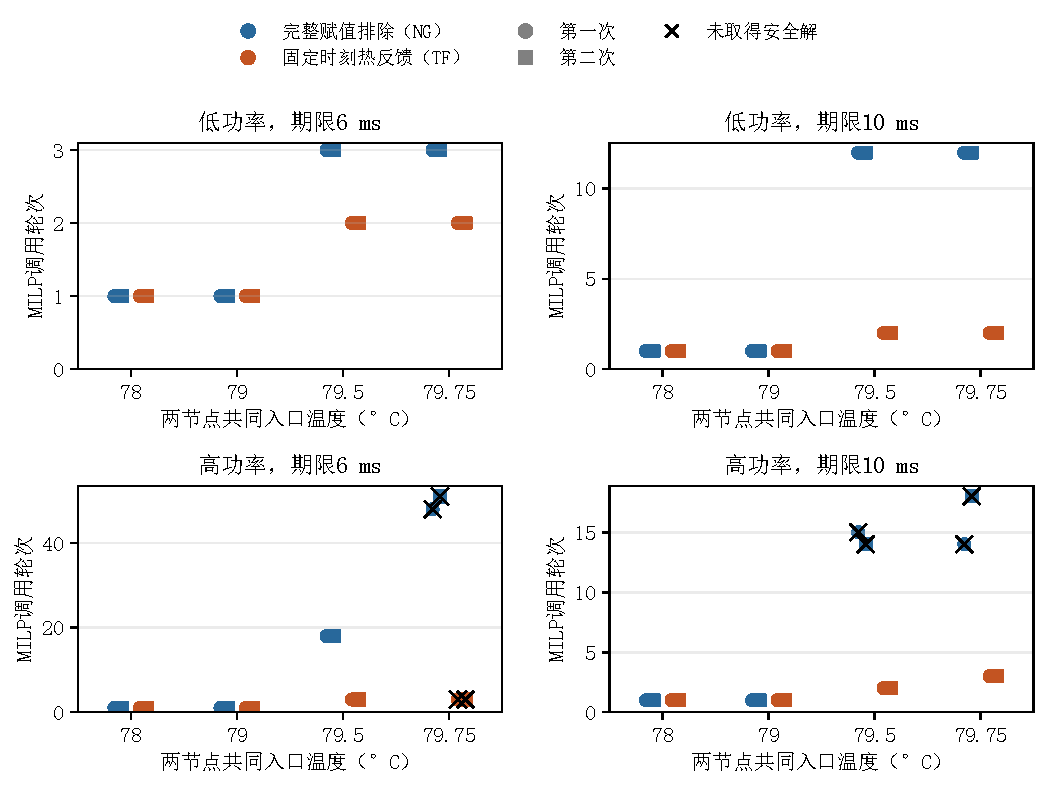
\includegraphics[width=\linewidth]{figures/pressure78_rounds.pdf}
\caption{预定入口热压力下两方法的MILP调用轮次。圆点、方点分别表示两次运行，叉号表示预算内没有安全输出；横向偏移只为避免遮挡。超时轮次是已发生的调用数，不表示搜索完成。各温度作为离散条件展示，不插值为连续区域边界。}
\label{fig:pressure-rounds}
\end{figure}

两方法各32次调用中，NG取得26次预算内安全输出，TF取得30次，其中达到独立下界的次数分别为12和16。双方均有安全输出的26个配对，能量全部相同。低功率包在79.5和79.75°C下的四个条件，以及高功率包6 ms、79.5°C条件，两次重复均减少求解轮次并缩短墙钟；例如低功率、10 ms的两档高温条件均由12轮减至2轮。这五个条件的最终时间表在方法之间有所不同，表明相同能量可以对应不同安全安排，不能将能量相同写成配置或时序相同。

高功率、10 ms、79.5与79.75°C进一步体现了预算内输出能力的差异。NG四次调用均超时且无安全$U$，TF分别用2轮和3轮取得42.625 mJ，并由$U=L_0$独立确定最优值。安全见证同时说明这些条件确实可行，NG未找到安排源于本次求解预算的限制。这里改善的是有限预算下取得有效答案的能力，不能为无输出方法补设能量，也不能据此计算节能率。

高功率、6 ms、79.75°C下，两方法均没有安全输出。NG两次超时，TF两次均在加入两条热行、完成3轮后由求解器报告无解。有效热行能够保留安全安排，但不能自行认证浮点求解器已完整排尽剩余整数域，因此该结果不构成独立热不可行证明。相应内部界及退出状态与安全$U$、独立$L_0$分别记录，不能相互替代。

入口较低的结果限定了反馈收益的适用条件。78与79°C共8个条件，两种方法的首候选均安全，全部一轮结束且零反馈；16个配对中TF恰有8次较快、8次较慢，不能把这些时间差归因于未执行的热行。两档较高初温的8个条件首候选均违规；全部32个配对的首候选选项集合相同，因而轮次差并非由不同初始候选造成。两次顺序平衡重复支持当前观察的一致性，但不足以估计方差、置信区间或跨平台的稳定加速。

信息复用的作用还体现在求解过程。正式组NG共生成240条完整赋值排除，TF生成22条热行且无回退；累计求解轮次由272降至54，不同候选及完整热评价次数由282降至56。一轮可能在回调中访问多个候选，因此轮次不能等同于候选数。全部保存轮次的求解器分支节点计数均为0，所观察到的减少是外层重复求解，不能表述为分支树节点减少。TF的约束构造累计约0.602 s，高于NG的0.042 s；在触发反馈且双方成功的五个条件中，这项新增成本由后续求解减少所抵消。

计时采用完整调用墙钟，首次安全获得时间另以外部时刻区间记录，并以上端判断预算准入；不将区间下端当作精确首解时刻。NG六次超时的实际返回时间为60.164--63.701 s，超出60 s的部分为停止延迟，未将晚形成的状态或内部界补记为预算内证据。各项时间由此包含真实停止成本，同时保持相同的有效预算。

另设高功率、6 ms、79.45°C发现性诊断，用于检查已有违规轨迹是否能在正常求解中触发反馈。该点根据既有轨迹构造，与正式温度组分开：两方法各运行一次，均自主取得44 mJ安全输出，NG为18轮、24.826 s，TF为3轮、4.205 s；独立$L_0$仍为42.625 mJ，故只记录安全见证与内部收敛。诊断结果不并入16个正式条件的成功率或重复统计。

上述结果将离线覆盖性质与完整求解中的条件性收益联系起来：当较高入口使正常候选违规时，固定时刻热行可将同一温度条件传回全部调度选项，减少重复尝试，并在部分受预算限制的调用中取得安全最优值见证。该作用未改变能耗模型，双方成功时也没有观察到能量下降；结论限于所列抽象参数、有限网格和求解器设置，不外推为真实设备节能或所有热调度实例的速度优势。


\subsection{结果讨论与适用范围}

模型验证表明，响应修正的系统价值受期限与资源限制，热约束可以收缩配置集合而不提高最低能量。方法验证进一步说明，连续温度违规信息可以形成有效线性约束，并在所测高入口条件下减少重复求解。表\ref{tab:evidence-map}列出各结论的证据来源，以免将模型关系、信息复用和计算效果混为一项结论。

\begin{table}[htbp]
\centering\small
\caption{验证问题、求解来源与证据范围}\label{tab:evidence-map}
\setlength{\tabcolsep}{4pt}
\begin{tabular}{@{}p{2.2cm}p{2.5cm}p{4.4cm}p{4.7cm}@{}}
\toprule
验证问题 & 求解来源 & 已有证据 & 尚不能支持的结论\\
\midrule
响应修正是否改变决策 & 解析下界、排除及见证核验 & 宽期限有能量差，紧期限不变；覆盖反比模型并列解的回放能量 & 不是两种响应的MILP直接配对运行，也不是实测精度验证\\
温度是否限制配置 & 完整网格枚举 & 104个最优配置保留80个，最低仍44 mJ & 不推出最低能量提高或连续启动域的配置排除\\
热行是否利用更多信息 & 完整合法域离线核对 & 单行排除16或32条违规安排，零误删安全安排 & 排除数量本身不等于MILP加速\\
接入是否必然触发 & 原输入上独立MILP对照 & 9项可行输入均首轮安全，全部零反馈 & 不能由未触发时的耗时差判断反馈价值\\
反馈是否改善求解 & 16条件、两方法、两次运行 & 安全输出26/32与30/32；5条件轮次及时间减少，2条件仅反馈取得安全解 & 不证明普遍加速、运行能耗下降或创新充分成立\\
\bottomrule
\end{tabular}
\end{table}

本章方法的增量在于：把完整轨迹中已确认的违规位置转换为全选项温度必要条件，并在可靠数值包络下传回MILP。它复用线性热模型和约束生成思想，针对本题的设备映射、频率与启动选项完成表达、有效性论证和求解验证；不将RC、查表或约束生成本身视为新原理。与只删除当前安排相比，实际收益还取决于求解器是否遇到违规候选、候选是否共享可复用的温度关系，以及构造约束的代价。

各组输入、时间表、结果及求解来源的复现索引见随稿材料\cite{artifact-index}。响应对照尚未改为MILP直接配对运行，当前解析证据仍按其来源保留。强化MILP与第四章有界搜索的比较也需使用相同输入、预算和连续热接纳条件；原来对完整赋值排除方法的比较不能替代这一比较。

模型的现实适用范围由数据与假设共同决定。公开工件提供了四Stage结构和作者报告的设备支持，尚没有同平台Lite0各Stage多频点时长、活动功率与RC配套测量。因此本章实验用于分析声明条件下的决策关系，不用于估计某款设备的实际节能率。冷热与期限对照也只覆盖所列条件，不能从有限案例推断现实系统的出现频率。

能量分解还依赖加性功率和固定模式响应。如果并发改变活动功率或执行时长，或温度泄漏、休眠和切换代价使能量依赖安排，目标一般需要恢复为$E(m,s)$。此时，一条安全时序不能确定该配置的最低能量，独立Stage下界也需重新检查，尤其不能忽略可能为负的并发修正。本文将这类情形作为适用边界，不并入当前模型和求解保证。

\clearpage
\section{本章小结}

本章围绕有限已知CPU--NPU推理请求，建立了任务相关响应下的联合调度模型。模式表统一表示设备、频率、时长和活动功率，依赖、资源及频率域限定合法安排，入口状态与节点功率轨迹共同决定连续温度。固定窗口与统一基准保证不同安排的能耗可比。

在上述假设下，配置决定活动能量，时序决定其能否在期限和热约束下实现。本章据此给出能量下界、配置可行域关系及有限网格MILP编码。针对逐条删除超温安排难以复用违规信息的问题，从具体违规节点与时刻构造全选项线性温度约束，证明其保留全部热安全安排，并给出相对完整赋值排除的整数域覆盖关系。最终接纳仍依赖完整连续热复核。

条件性实验从两个层面支撑上述工作。模型层面，宽期限下响应修正改变可实现系统能量，紧期限下选择也可以不变；温度能够排除部分原最优配置而不提高最低能量。方法层面，热行在完整合法域核对中扩大排除范围且未误删安全安排；原输入均未触发反馈，而预定热压力组中安全输出由26/32次增至30/32次，部分条件减少了求解轮次与时间。双方均成功时能量相同，结果支持限定条件下的求解收益，不外推为实际设备节能或普遍速度优势。

第四章沿用同一模型与安全标准，研究配置能量下界引导的有界搜索，并与本章热反馈MILP比较相同预算内的安全解质量、可核查界和计算表现。
